\documentclass[journal,11pt]{IEEEtran}

% --- Codificación e idioma ---
\usepackage[utf8]{inputenc}
\usepackage[T1]{fontenc}
\usepackage[spanish,es-nodecimaldot,es-tabla]{babel}

% --- Gráficos, matemáticas y tablas ---
\usepackage{graphicx}
\usepackage{amsmath,amssymb,amsfonts}
\usepackage{booktabs}
\usepackage{tabularx}
\usepackage{array}
\usepackage{cite}
\usepackage{microtype}
\usepackage{tikz}
\usetikzlibrary{arrows.meta,positioning,babel}

\graphicspath{{./}{./Figuras/}}

\renewcommand{\figurename}{Fig.}

% --- Atajos ---
\newcommand{\pct}{\ifmmode\mskip\thinmuskip\mathchar"0025\relax\else\,\char37\relax\fi}
\newcommand{\pC}[1]{\ensuremath{#1\mskip\thinmuskip\mathchar"0025\mskip\thinmuskip\mathrm{C}}}
\newcommand{\FeFeC}{Fe--Fe$_3$C}

\begin{document}

% ==============================================================================
% TÍTULO Y AUTORES
% ==============================================================================
\title{Identificación y Análisis Microestructural de Aceros, Fundiciones de Hierro y Tratamientos Térmicos\\[3pt]
\large\textit{Microstructural Identification and Analysis of Steels, Cast Irons and Heat Treatments}}

\author{
    \IEEEauthorblockN{
        Juan José Tobar Álvarez,
        Angélica Plata Martínez,
        Sergio Correales Sarmiento, \\
        Daniel Alejandro Carvajal Guecha y
        Paula Stephania Pérez Gil
    }\\
    \IEEEauthorblockA{
        \textit{Departamento de Ingeniería Mecánica y Mecatrónica, Facultad de Ingeniería}\\
        \textit{Universidad Nacional de Colombia, Sede Bogotá}\\
        \textit{Ciencia e Ingeniería de Materiales (2017256-1), Grupo 01}\\
        \textit{Prof. Jhon Jairo Olaya Flórez --- Práctica de Microestructura, 23 de noviembre de 2026}\\
        Email: \{jutobara, anplatam, scorreales, dcarvajalgu, pperezgi\}@unal.edu.co
    }
}

\maketitle

% ==============================================================================
% RESUMEN
% ==============================================================================
\begin{abstract}
La microestructura de las aleaciones ferrosas determina sus propiedades mecánicas y depende de su composición y de su historia térmica. Este trabajo tuvo como objetivo identificar, mediante microscopía óptica de luz reflejada, las inclusiones no metálicas y las microestructuras de aceros al carbono (hierro puro, AISI 1005, 1020, 1045, 1060 y 1080), aceros aleados (4340 en estado de entrega, templado y templado con revenido; 8620 y H13) y fundiciones de hierro (gris y blanca), y relacionarlas con el diagrama \FeFeC. Las probetas se observaron primero sin ataque, para evaluar las inclusiones según la norma ASTM E45, y luego atacadas con Nital; las observaciones se registraron en apuntes y esquemas morfológicos, sin captura de imágenes. Se identificaron óxidos globulares y sulfuros alargados; ferrita de granos alargados en el hierro puro y equiaxiales en el AISI 1005; un aumento progresivo de la perlita con el contenido de carbono, cuya proporción teórica según la regla de la palanca pasa de $\approx 4\pct$ (AISI 1005) a $\approx 100\pct$ (AISI 1080); grafito laminar en la fundición gris y ledeburita en la blanca; y estructuras de temple, cementación y carburos en los aceros aleados. Se concluye que el carbono controla la fracción de perlita y que los tratamientos térmicos y termoquímicos modifican de forma drástica la microestructura; la cuantificación experimental de fases queda como trabajo futuro.
\end{abstract}

\begin{IEEEkeywords}
Microscopía metalográfica, ataque químico, inclusiones, regla de la palanca, ferrita, perlita, martensita, fundiciones.
\end{IEEEkeywords}

% ==============================================================================
% INTRODUCCIÓN
% ==============================================================================
\section{Introducción}
\IEEEPARstart{L}{a} metalografía estudia la constitución estructural de los metales y aleaciones y permite relacionar el procesamiento mecánico y térmico de un material con su comportamiento en servicio \cite{smith}. El análisis microestructural con microscopía óptica de luz reflejada es la técnica más accesible para evaluar la calidad de una aleación, estimar sus propiedades mecánicas y diagnosticar fallas.

En las aleaciones ferrosas, las propiedades dependen de las fases presentes (ferrita, cementita, perlita, martensita), del tamaño y la forma del grano y de las impurezas inevitables conocidas como inclusiones no metálicas \cite{callister}. Estas inclusiones, como óxidos y sulfuros, se originan durante la desoxidación y la solidificación del acero; su forma, cantidad y distribución alteran la isotropía del material y pueden actuar como concentradores de esfuerzos que favorecen la falla por fatiga o impacto \cite{ashby2}.

El orden de revelado es crítico en la preparación metalográfica: las inclusiones deben evaluarse con la probeta en condición de pulido espejo (sin ataque), porque el ataque químico degrada la matriz y puede ocultarlas o confundirlas con picaduras \cite{shackelford,astm_e3}. Después, un reactivo como el Nital (ácido nítrico en etanol) revela los límites de grano y los constituyentes al atacar de forma selectiva zonas de distinta reactividad \cite{astm_e407}.

\textbf{Antecedentes.} Los textos de referencia establecen tres relaciones que esta práctica permite comprobar de forma cualitativa: (i) en aceros hipoeutectoides la fracción de perlita crece de forma casi lineal con el contenido de carbono hasta $0.77\pct$ C \cite{callister}; (ii) en las fundiciones, el carbono aparece como grafito (fundición gris) o como cementita (fundición blanca) según la composición y la velocidad de enfriamiento; y (iii) el temple produce martensita dura y frágil que requiere revenido para recuperar tenacidad \cite{callister,asm9}.

\textbf{Trabajos recientes.} La caracterización microestructural de aceros aleados y fundiciones sigue siendo un tema activo. Clarke \textit{et al.} estudiaron el AISI 4340 templado y revenido con técnicas de caracterización a varias escalas y mostraron que el revenido a baja temperatura alivia la sobresaturación de carbono de la martensita mediante carburos de transición; además, vinculan la fragilización por revenido de la martensita, que aparece entre 200 y 400~$^{\circ}$C aproximadamente, con la descomposición de la austenita retenida \cite{clarke}. En el acero para trabajo en caliente H13, Ning \textit{et al.} observaron con microscopía óptica y electrónica de transmisión una matriz martensítica con carburos MC y M$_6$C menores de 200~nm y carburos M$_{23}$C$_6$ de mayor tamaño, y atribuyeron el endurecimiento secundario principalmente a los primeros \cite{ning}. Para las fundiciones, Vaško señala que la microscopía óptica de luz reflejada permite distinguir la forma del grafito (laminar, vermicular o nodular) y la matriz, que el Nital es el reactivo más empleado y que la solidificación eutéctica de la fundición blanca sigue el diagrama metaestable \FeFeC{} y produce ledeburita \cite{vasko}. Estos trabajos respaldan las morfologías que se buscan reconocer aquí: martensita revenida en el 4340, carburos en el H13 y grafito laminar o ledeburita en las fundiciones.

\textbf{Aporte.} Este informe reúne, en un esquema comparativo único, la secuencia de observación (sin ataque $\rightarrow$ con ataque) y las microestructuras típicas de aceros al carbono, aceros aleados tratados y fundiciones, relacionándolas con el diagrama \FeFeC{} y con una estimación teórica de fases.

\subsection{Objetivos}
\begin{itemize}
    \item Identificar y clasificar inclusiones no metálicas en aceros sin ataque según la norma ASTM E45 \cite{astm_e45}, distinguiendo óxidos (redondeados) de sulfuros (alargados).
    \item Diferenciar las microestructuras del hierro puro y de los aceros AISI 1005, 1020, 1045, 1060 y 1080, y comparar la proporción de perlita observada con la que predice la regla de la palanca.
    \item Interpretar el concepto de ``estado de entrega'' del acero AISI 4340.
    \item Caracterizar las fundiciones gris y blanca \cite{astm_a247} y el efecto del temple, el revenido y la cementación (aceros 4340 y 8620), así como la presencia de carburos en el acero H13.
\end{itemize}
La metodología consistió en observar cada probeta en dos etapas (sin ataque y con ataque de Nital) y registrar la morfología mediante apuntes y esquemas.

% ==============================================================================
% DESARROLLO EXPERIMENTAL
% ==============================================================================
\section{Desarrollo Experimental}
La secuencia seguida se resume en la Fig.~\ref{fig:diagrama_flujo}. Por restricciones del laboratorio no se tomaron fotografías; la información se registró en apuntes morfológicos y esquemas, y por ello las figuras de este informe son esquemas ilustrativos y no micrografías.

\begin{figure}[!t]
\centering
\begin{tikzpicture}[node distance=0.55cm,
    block/.style={draw, fill=blue!8, text width=6.9cm, align=center, minimum height=0.7cm, rounded corners=2pt, font=\scriptsize},
    line/.style={-{Latex[length=2mm]}, thick}]
    \node [block] (prep) {1. Preparación de probetas (corte, desbaste y pulido espejo)};
    \node [block, below=of prep] (inc) {2. Observación \textbf{sin ataque}: inclusiones (óxidos redondeados y sulfuros alargados; ASTM E45)};
    \node [block, below=of inc] (ataque) {3. Ataque químico con Nital};
    \node [block, below=of ataque] (micro) {4. Observación \textbf{con ataque}: ferrita, perlita, martensita, grafito y carburos (apuntes y esquemas)};
    \node [block, below=of micro] (analisis) {5. Correlación con el diagrama \FeFeC{} y la regla de la palanca};
    \foreach \a/\b in {prep/inc, inc/ataque, ataque/micro, micro/analisis} \draw [line] (\a) -- (\b);
\end{tikzpicture}
\caption{Secuencia experimental para identificar inclusiones y microestructura.}
\label{fig:diagrama_flujo}
\end{figure}

\subsection{Fundamentos Teóricos}
La microscopía óptica de luz reflejada (epi-iluminación) se fundamenta en la reflexión diferencial que experimenta un haz incrustado de luz visible al incidir sobre la superficie especular de un material opaco. El contraste de las fases depende de las variaciones de reflectividad óptica y de la topografía microestructural generada durante la preparación.

El ataque químico selectivo aprovecha la diferencia de potencial electroquímico y de energía libre interfacial entre los constituyentes de la aleación. Al emplear Nital (solución de ácido nítrico en etanol), las moléculas del ácido disuelven preferentemente la ferrita ($\alpha$) y atacan las zonas de alta densidad energética, como los límites de grano y las interfaces interlaminares de la perlita. Esta disolución diferencial crea microsurcos topográficos. La luz que incide en estos surcos e interfaces se dispersa fuera del cono de captación del objetivo, observándose zonas oscuras en campo claro. Por el contrario, fases más nobles o insolubles (como la cementita, $\mathrm{Fe_3C}$) no reaccionan y permanecen planas y brillantes por reflexión directa.

\subsection{Material}
Se analizaron aceros al carbono (hierro puro y AISI 1005, 1020, 1045, 1060 y 1080), aceros aleados (AISI 4340 en estado de entrega, templado y templado con revenido; 8620 y H13) y fundiciones de hierro (gris y blanca eutéctica). Las composiciones nominales de carbono se indican en la Tabla~\ref{tab:resumen_muestras}.

\subsection{Equipos}
Las observaciones se hicieron en dos microscopios metalográficos de luz reflejada, necesarios para materiales opacos (Fig.~\ref{fig:microscopio}), que los apuntes de laboratorio identifican como microscopio (1) y microscopio (2): (1) Olympus GX41, invertido, con cámara Zeiss Axiocam 105 color acoplada al tubo trinocular (no utilizada para captura de imágenes en esta práctica), y (2) Zeiss Primotech, con selector de iluminación transmitida (TL) y reflejada (RL) y un revólver con objetivos Zeiss A-Plan de $5\times$ y $63\times$ y EC Epiplan de $50\times$. La operación de los equipos estuvo a cargo del técnico del laboratorio; las probetas se observaron en campo claro con luz reflejada.
El haz de la fuente atraviesa la lente condensadora y el diafragma, se desvía hacia la probeta mediante un espejo semitransparente a $45^{\circ}$ y, tras reflejarse en la superficie, regresa por el objetivo y el espejo hasta el ocular. El aumento total es el producto del aumento del objetivo por el del ocular ($10\times$): los aumentos registrados fueron $200\times$ (acero H13) y $500\times$ (AISI 1080), obtenidos con objetivos de $20\times$ y $50\times$, respectivamente.

\begin{figure}[!t]
\centering
\begin{tikzpicture}[>=Latex,font=\scriptsize,
  box/.style={draw,rounded corners=1.5pt,align=center,inner sep=2.5pt,minimum height=0.6cm},
  inc/.style={orange!85!black,dashed,thick,->},
  ref/.style={red!75!black,thick,->}]
  \def\xc{4.4}
  \draw[inc] (1.15,3.55)--(\xc-0.1,3.55)--(\xc-0.1,1.1);
  \draw[ref] (\xc+0.1,1.0)--(\xc+0.1,4.75);
  \draw[blue!60!black,line width=2pt] (\xc-0.4,3.85)--(\xc+0.4,3.05);
  \node[box,fill=violet!12] at (\xc,5.15) {Ocular ($10\times$)};
  \node[box,fill=green!12,minimum width=2.3cm] at (\xc,1.95) {Objetivo\\($20\times$, $50\times$)};
  \node[draw,fill=gray!25,minimum width=3.4cm,minimum height=0.4cm] at (\xc,0.7) {Probeta pulida / atacada};
  \node[draw,fill=gray!65,text=white,minimum width=4.0cm,minimum height=0.4cm] at (\xc,0.25) {Platina móvil (X--Y)};
  \node[box,fill=orange!15] at (0.5,3.55) {Fuente\\de luz};
  \draw[fill=blue!15] (1.85,3.55) ellipse (0.09 and 0.42);
  \node[align=center] at (1.85,4.3) {Lente\\condensadora};
  \draw[very thick] (3.0,4.0)--(3.0,3.75); \draw[very thick] (3.0,3.35)--(3.0,3.1);
  \node[align=center] at (3.0,2.65) {Diafragma};
  \node[align=left,anchor=west] (esp) at (5.35,4.15) {Espejo\\semitransparente\\($45^{\circ}$)};
  \draw[->,blue!60!black] (esp.south west)++(0.02,0.05) to[bend right=12] (\xc+0.3,3.2);
  \node[anchor=west,align=left] at (5.35,5.15) {Aumento total:\\$200\times$--$500\times$};
  \draw[inc] (0.1,5.2)--(0.7,5.2); \node[anchor=west] at (0.75,5.2) {Haz incidente};
  \draw[ref] (0.1,4.85)--(0.7,4.85); \node[anchor=west] at (0.75,4.85) {Haz reflejado};
\end{tikzpicture}
\caption{Esquema óptico de luz reflejada (configuración vertical, como en el Zeiss Primotech). En el Olympus GX41, invertido, la probeta se apoya con la cara pulida hacia abajo y el objetivo queda debajo de ella.}
\label{fig:microscopio}
\end{figure}

\subsection{Procedimiento}
Las probetas fueron preparadas por el personal técnico del laboratorio según la práctica metalográfica convencional (corte, desbaste y pulido hasta acabado espejo) \cite{astm_e3,asm9}.
Los parámetros de preparación (abrasivos y tiempos de desbaste y pulido) y de ataque (concentración del Nital y tiempo de inmersión) no fueron suministrados durante la práctica y por ello no se reportan; los rótulos ``Nital 2\pct'' de los esquemas indican una concentración típica de referencia (en la literatura se emplean concentraciones de 1 a 4\pct\ \cite{vasko}), no un dato medido.
Cada probeta se observó primero \emph{sin ataque} para evaluar las inclusiones y después se atacó con Nital. Este reactivo disuelve preferentemente los límites de grano y la ferrita, de modo que la cementita queda en relief; la perlita laminar dispersa la luz y se ve oscura frente a la ferrita clara. Se registraron la morfología de cada fase y, para el AISI 1080 ($500\times$) y el H13 ($200\times$), el aumento utilizado.

\subsection{Estimación teórica de fases}
Para un acero hipoeutectoide con contenido de carbono $C_0$ ($C_0<0.77\pct$), la fracción de perlita se obtiene aplicando la regla de la palanca sobre la línea de reparto a $727\,^{\circ}$C (Fig.~\ref{fig:diagrama_fe_fe3c}b):
\begin{equation}
    f_P=\frac{C_0-C_\alpha}{C_P-C_\alpha}\times100,\qquad f_{\alpha'}=100-f_P,
    \label{eq:palanca}
\end{equation}
con $C_\alpha=0.022\pct$ (solubilidad máxima del carbono en la ferrita) y $C_P=0.77\pct$ (composición eutectoide) \cite{callister}. Esta estimación supone enfriamiento lento (equilibrio) y $f_{\alpha'}$ es la ferrita proeutectoide, que aparece clara bajo el microscopio.

% ==============================================================================
% RESULTADOS Y DISCUSIÓN
% ==============================================================================
\section{Resultados y Discusión}

\subsection{Inclusiones no metálicas (sin ataque)}
En estado de pulido espejo (Fig.~\ref{fig:series_carbono}a) se distinguieron dos morfologías:
\begin{itemize}
    \item \textbf{Partículas redondeadas (óxidos)}: inclusiones globulares oscuras y aisladas (tipo D de ASTM E45), generalmente óxidos complejos de silicio, aluminio o hierro. No se deforman en el conformado en caliente por su dureza y fragilidad.
    \item \textbf{Partículas alargadas (sulfuros)}: inclusiones de sulfuro de manganeso (MnS, tipo A) orientadas en la dirección de laminado o forjado; al ser dúctiles a alta temperatura se deforman junto con la matriz \cite{ashby2}.
\end{itemize}
La clasificación se realiza por comparación con las tablas de la norma ASTM E45 \cite{astm_e45}, que distingue los tipos A (sulfuros), B (aluminatos), C (silicatos) y D (óxidos globulares). Dos observaciones del laboratorio refuerzan la conveniencia de evaluar primero sin ataque: la contabilización de inclusiones puede dificultarse porque algunas quedan ocultas, y tras el ataque aparecen puntos muy negros que corresponden a corrosión (picaduras) de la probeta y no a inclusiones. Distinguirlos solo es posible si se conoce el estado previo al ataque.

\begin{figure*}[!t]
\centering
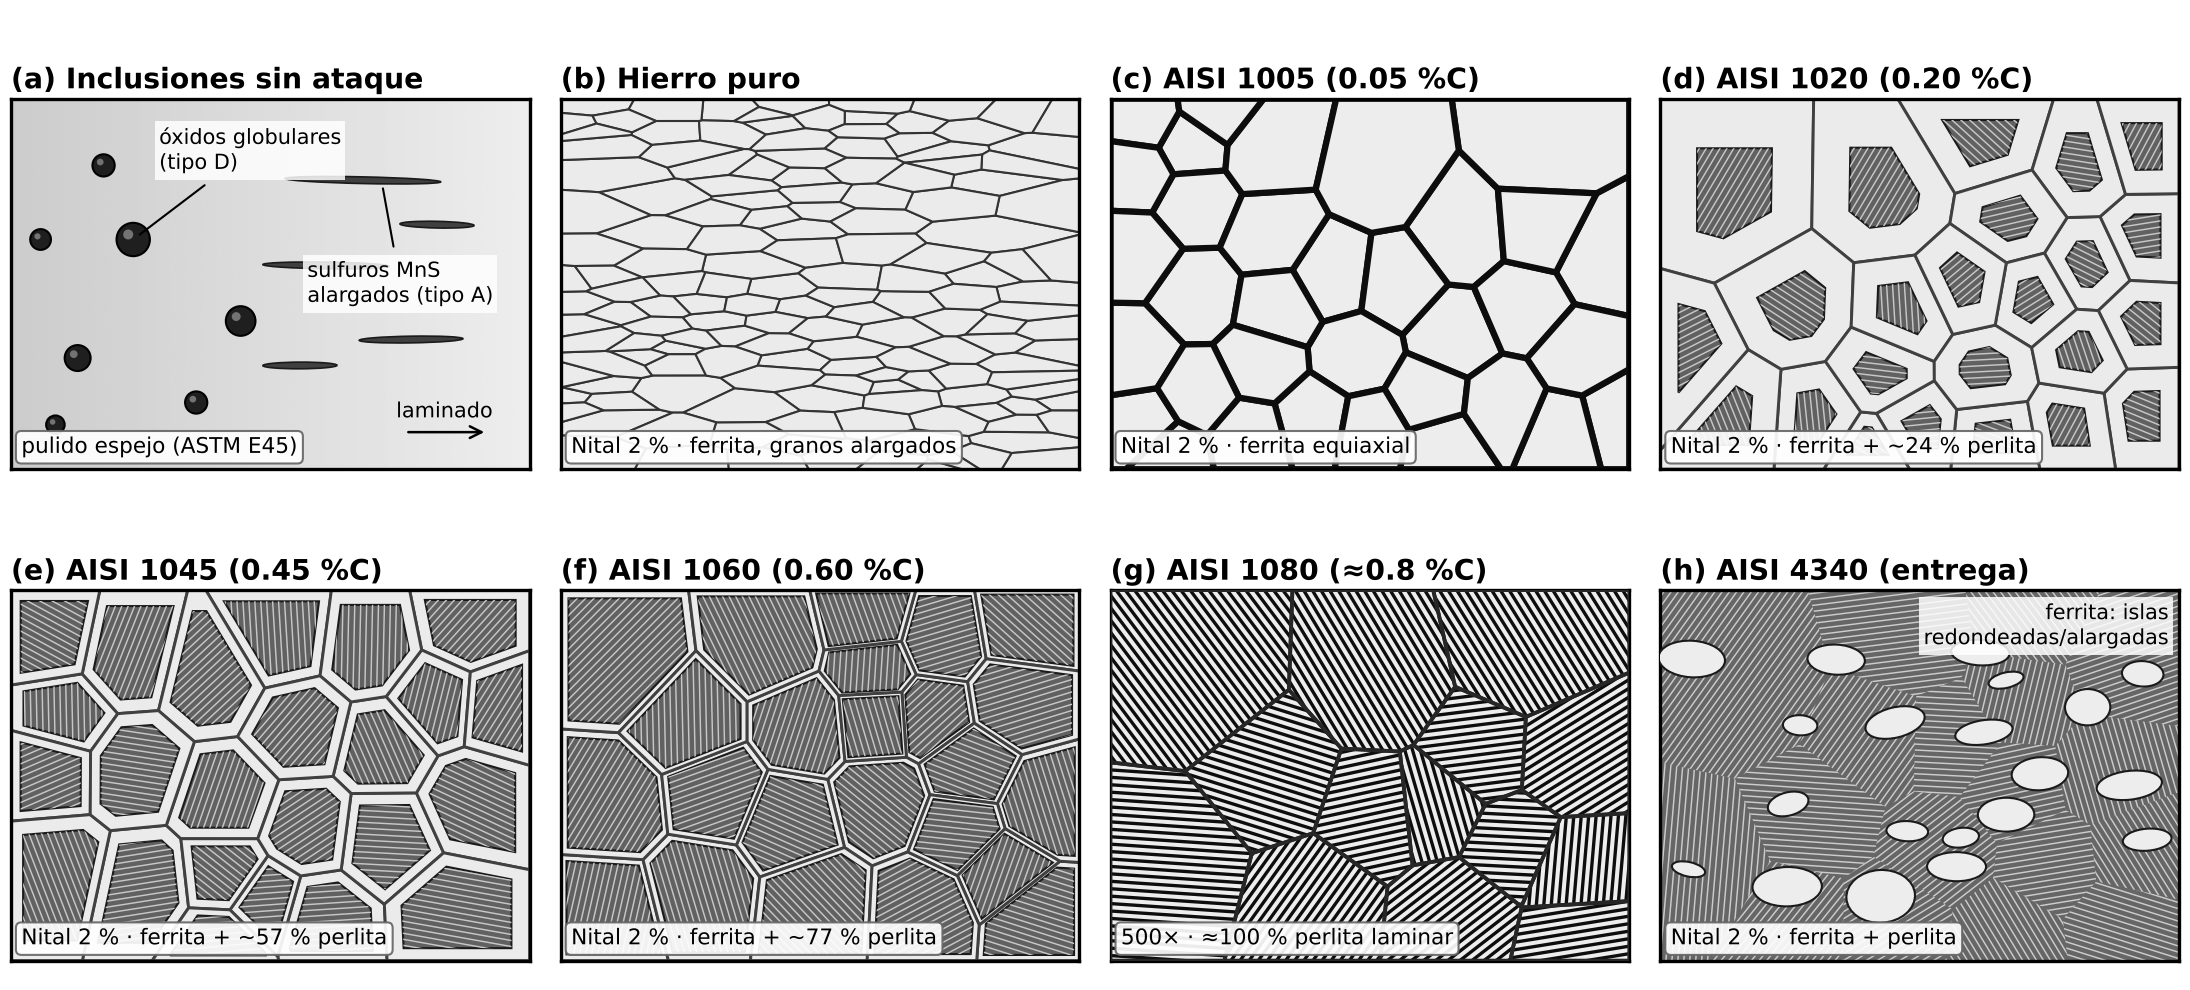
\includegraphics[width=\textwidth]{fig_series_carbono.png}
\caption{Esquemas ilustrativos de las morfologías registradas en el laboratorio (no son micrografías). (a) Inclusiones sin ataque; (b)--(g) aceros al carbono atacados con Nital en orden creciente de carbono, con la proporción teórica de perlita; (h) AISI 4340 en estado de entrega. Solo el AISI 1080 ($500\times$) tiene un aumento registrado.}
\label{fig:series_carbono}
\end{figure*}

\subsection{Aceros al carbono}
La Fig.~\ref{fig:series_carbono}b--g muestra la evolución observada. El \textbf{hierro puro} presentó granos de ferrita más alargados y una mayor densidad de granos; el \textbf{AISI 1005} ($\pC{0.05}$) mostró ferrita de granos equiaxiales con límites oscuros. Con el \textbf{AISI 1020} ($\pC{0.20}$) aparecen zonas oscuras de perlita sobre la matriz clara de ferrita, que crecen en el \textbf{AISI 1045} ($\pC{0.45}$) y predominan en el \textbf{AISI 1060} ($\pC{0.60}$), donde la ferrita queda como regiones claras discontinuas. En el \textbf{AISI 1080} ($\approx\pC{0.8}$), observado a $500\times$, la estructura es casi totalmente perlita y se resuelve su carácter laminar. El contraste se debe a la dispersión de la luz en el relieve que el ataque deja en la perlita \cite{callister}; por eso solo a mayores aumentos se distinguen las láminas.

Estas tendencias concuerdan con la regla de la palanca (Fig.~\ref{fig:diagrama_fe_fe3c}, Fig.~\ref{fig:palanca} y Tabla~\ref{tab:resumen_muestras}): la ecuación~\eqref{eq:palanca} predice $\approx4\pct$ de perlita en el AISI 1005, $24\pct$ en el 1020, $57\pct$ en el 1045, $77\pct$ en el 1060 y $\approx100\pct$ en el 1080. \textbf{Estos porcentajes son teóricos}: no se midió la fracción de perlita en las probetas, por lo que la comparación es cualitativa. La ferrita equiaxial del AISI 1005 y la alargada del hierro puro son ejemplos de los tamaños y formas de grano que se caracterizan con ASTM E112 \cite{astm_e112}.

\begin{figure*}[!t]
\centering
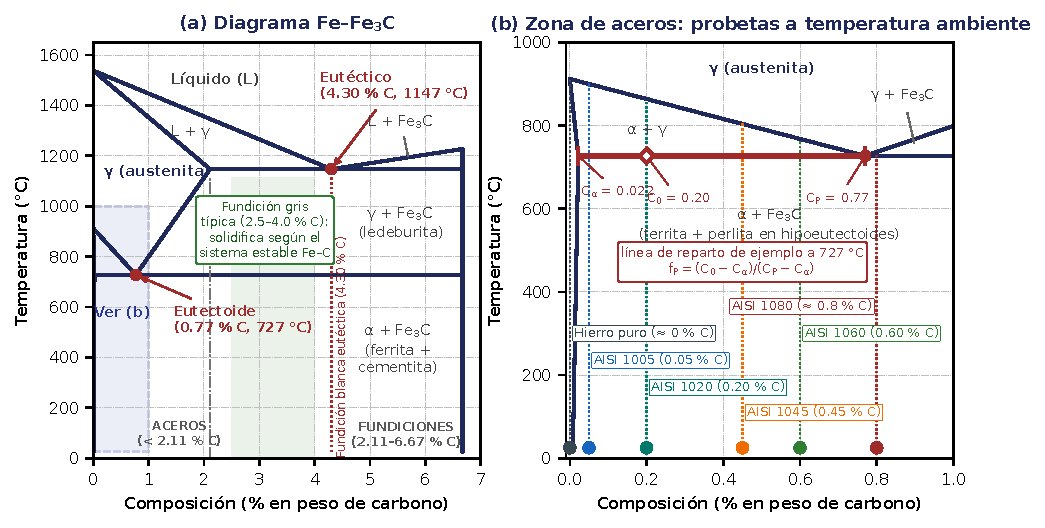
\includegraphics[width=\textwidth]{fig_fe_fe3c.pdf}
\caption{Diagrama de equilibrio metaestable \FeFeC{} simplificado (se omiten la región $\delta$ y la reacción peritéctica). (a) Diagrama completo; (b) zona de aceros con las probetas de acero al carbono ubicadas a temperatura ambiente y una línea de reparto de ejemplo ($C_0=0.20\pct$). Los aceros aleados no se ubican porque sus transformaciones no se describen con este diagrama; la fundición gris solidifica según el sistema estable Fe--C (grafito).}
\label{fig:diagrama_fe_fe3c}
\end{figure*}

\begin{figure*}[!t]
\centering
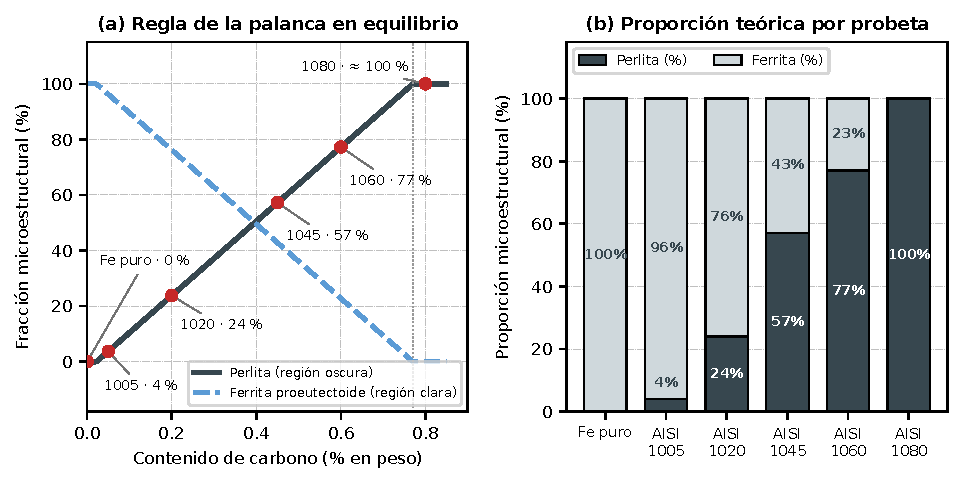
\includegraphics[width=\textwidth]{fig_palanca.pdf}
\caption{Regla de la palanca para los aceros al carbono evaluados ($C_\alpha=0.022\pct$, $C_P=0.77\pct$). (a) Fracción de perlita y de ferrita proeutectoide en función del carbono; (b) proporción teórica por probeta. Los valores son teóricos (equilibrio) y no mediciones experimentales.}
\label{fig:palanca}
\end{figure*}

\begin{table*}[!t]
\centering
\caption{Resumen microestructural de las probetas. Las fracciones P/F son teóricas (perlita/ferrita proeutectoide, ecuación~\eqref{eq:palanca}); en aceros aleados y fundiciones no se calculan.}
\label{tab:resumen_muestras}
\renewcommand{\arraystretch}{1.2}
\footnotesize
\begin{tabularx}{\textwidth}{@{} >{\raggedright\arraybackslash}p{3.1cm} c >{\raggedright\arraybackslash}p{3.4cm} >{\raggedright\arraybackslash}X c @{}}
\toprule
\textbf{Material / probeta} & \textbf{\% C} & \textbf{Condición registrada} & \textbf{Microestructura observada} & \textbf{P / F (\%)} \\ \midrule
Inclusiones (aceros) & variable & Sin ataque (pulido espejo) & Óxidos globulares (tipo D) y sulfuros MnS alargados (tipo A) & --- \\
Hierro puro & $\approx 0$ & Nital & Ferrita con granos alargados y mayor densidad de granos & 0 / 100 \\
AISI 1005 & 0.05 & Nital & Ferrita equiaxial con límites de grano oscuros & 4 / 96 \\
AISI 1020 & 0.20 & Nital & Matriz ferrítica clara con perlita oscura & 24 / 76 \\
AISI 1045 & 0.45 & Nital & Perlita y ferrita proeutectoide en proporción similar & 57 / 43 \\
AISI 1060 & 0.60 & Nital & Perlita mayoritaria con ferrita residual & 77 / 23 \\
AISI 1080 ($500\times$) & $\approx 0.8$ & Nital & Perlita laminar & $\approx$ 100 / 0 \\
AISI 4340 & 0.40 & Estado de entrega & Ferrita en islas redondeadas/alargadas y perlita & --- \\
AISI 4340 & 0.40 & Temple (tratamiento no aceptable) & Martensita acicular sin revenir & --- \\
AISI 4340 & 0.40 & Templado y revenido & Martensita revenida de aspecto fino y denso con austenita retenida & --- \\
AISI 8620 & 0.20 & Cementado & Capa martensítica superficial y núcleo ferrítico-perlítico & --- \\
Acero H13 ($200\times$) & 0.40 & --- & Matriz martensítica con carburos de cromo blancos y alargados & --- \\
Fundición gris & 2.5--4.0 (típ.) & Nital & Grafito laminar (flake) & --- \\
Fundición blanca eutéctica & 4.30 & Nital & Ledeburita; cementita blanca & --- \\ \bottomrule
\end{tabularx}
\end{table*}

\subsection{El estado de entrega del acero AISI 4340}
El ``estado de entrega'' es la condición microestructural y mecánica en la que el proveedor suministra el material, que por lo general corresponde a la \textbf{menor dureza posible} para facilitar el corte y el mecanizado antes de que el usuario aplique los tratamientos de endurecimiento. El AISI 4340 ($\approx\pC{0.40}$) mostró ferrita en forma de islas redondeadas que se ven alargadas, dentro de una matriz perlítica (Fig.~\ref{fig:series_carbono}h), estructura blanda y apta para mecanizar. Al ser un acero aleado, el diagrama \FeFeC{} solo describe su comportamiento de forma aproximada.

\subsection{Fundiciones de hierro}
En la \textbf{fundición gris} el carbono se presenta como grafito, una forma alotrópica del carbono, con varias morfologías que se clasifican según su forma (norma ASTM A247 \cite{astm_a247}); en la probeta se observó grafito alargado en hojuelas (Fig.~\ref{fig:especiales}a). El grafito libre favorece la maquinabilidad y el amortiguamiento, pero reduce la tenacidad. En la \textbf{fundición blanca}, de tipo eutéctico, el carbono forma cementita y la estructura se ve blanca (Fig.~\ref{fig:especiales}b): corresponde a ledeburita, el eutéctico de austenita y cementita (a temperatura ambiente, la austenita se ha transformado, típicamente en perlita), y es muy dura y frágil. Que una composición similar produzca grafito o cementita depende de la velocidad de enfriamiento y de elementos como el silicio.

\begin{figure*}[!t]
\centering
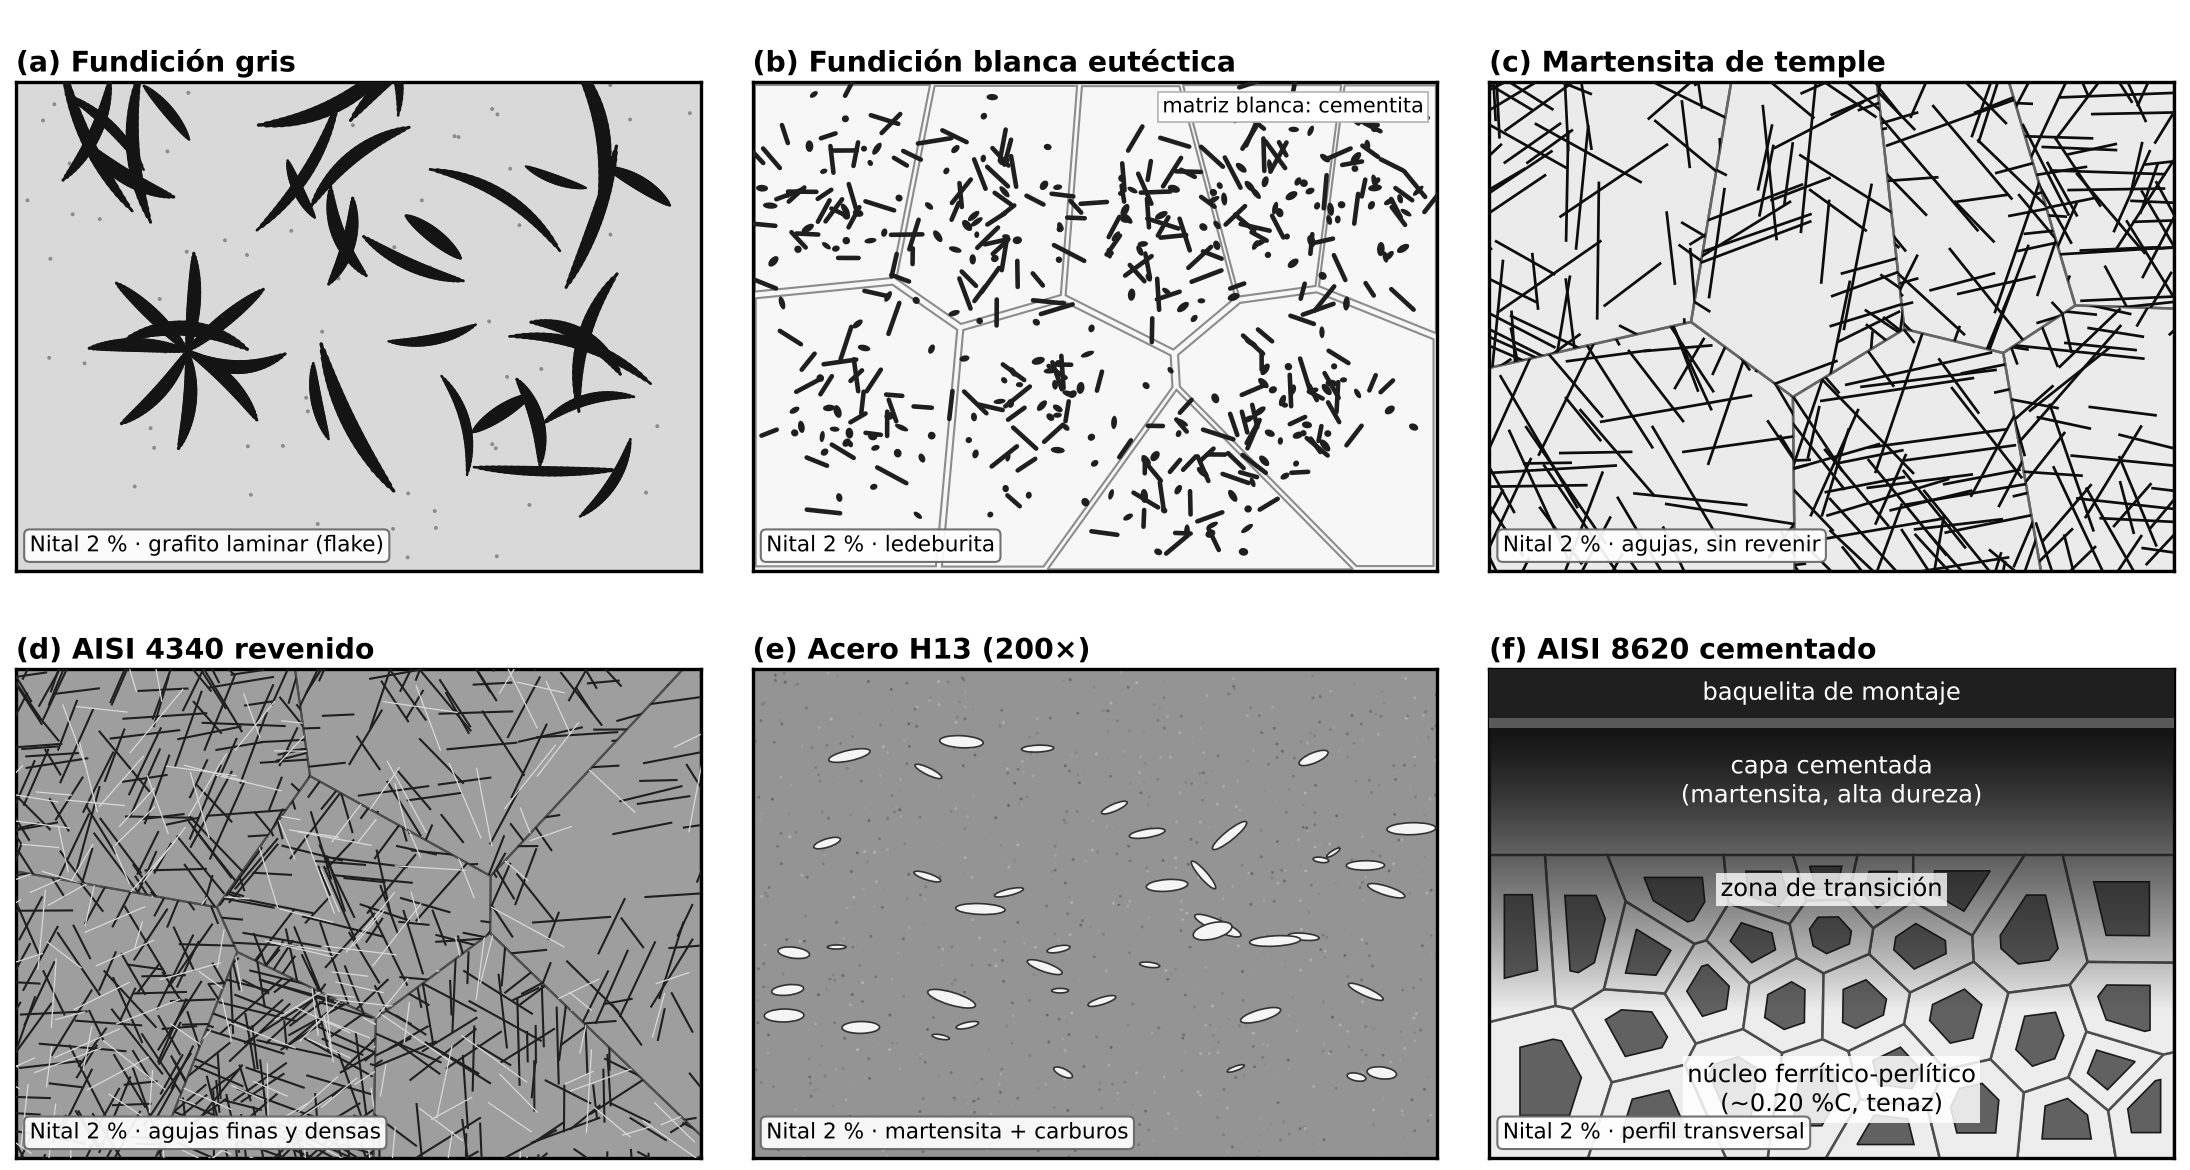
\includegraphics[width=\textwidth]{fig_estructuras_especiales.png}
\caption{Esquemas ilustrativos de las morfologías registradas (no son micrografías). (a) Fundición gris con grafito laminar; (b) fundición blanca eutéctica con ledeburita; (c) martensita de temple sin revenir (AISI 4340 templado); (d) martensita revenida (AISI 4340 templado y revenido); (e) acero H13 ($200\times$) con carburos blancos alargados; (f) perfil transversal del acero 8620 cementado.}
\label{fig:especiales}
\end{figure*}

\subsection{Estructuras fuera de equilibrio y tratamientos térmicos}
\begin{itemize}
    \item \textbf{Martensita de temple (AISI 4340).} El temple produjo martensita en agujas (Fig.~\ref{fig:especiales}c). Sin revenido es muy dura pero frágil y con tensiones residuales, por lo que el tratamiento se consideró no aceptable para servicios que exigen tenacidad \cite{callister}.
    \item \textbf{Martensita revenida (AISI 4340).} El mismo acero, templado y revenido, muestra una morfología de agujas finas y densas (Fig.~\ref{fig:especiales}d); el revenido alivia tensiones y mejora la tenacidad a costa de parte de la dureza \cite{callister,asm9}. En esta probeta se identificó además la presencia de austenita retenida junto a las agujas martensíticas, lo que evidencia una transformación martensítica incompleta durante el temple rápido previo y su posterior descomposición parcial en constituyentes más estables durante el calentamiento de revenido \cite{clarke}. Así, el AISI 4340 se observó en tres condiciones (entrega, temple y temple con revenido), lo que permite comparar directamente el efecto del tratamiento sobre un mismo material.
    \item \textbf{Acero 8620 cementado.} Se observó un gradiente (Fig.~\ref{fig:especiales}f): la baquelita de montaje, una zona de cementación martensítica superficial y un núcleo ferrítico-perlítico ($\approx\pC{0.20}$). Esta combinación (superficie dura, núcleo tenaz) es el objetivo del tratamiento termoquímico.
    \item \textbf{Acero H13 ($200\times$).} Sobre una matriz martensítica se distinguieron estructuras blancas alargadas, que corresponden a carburos de cromo propios de los aceros para herramientas (Fig.~\ref{fig:especiales}e). El H13 es un acero Cr--Mo--V de trabajo en caliente cuyos carburos aportan resistencia al desgaste y dureza en caliente \cite{asm9}.
\end{itemize}

\subsection{Limitaciones}
No se capturaron imágenes ni se midieron fracciones de fase, de modo que las comparaciones con la regla de la palanca y con la bibliografía son cualitativas, y las fracciones de la Tabla~\ref{tab:resumen_muestras} suponen equilibrio, sin considerar el estado de suministro ni el tratamiento previo de cada probeta, que no se registraron. Tampoco se registraron los parámetros de preparación y de ataque (abrasivos, pulido, concentración del Nital y tiempo de ataque), lo que limita la reproducibilidad. Para cuantificar se recomienda tomar micrografías y aplicar conteo manual de puntos (ASTM E562 \cite{astm_e562}) o análisis de imagen, y registrar el estado de suministro de cada probeta.

% ==============================================================================
% CONCLUSIONES
% ==============================================================================
\section{Conclusiones}
\begin{enumerate}
    \item El contenido de carbono controla la fracción de perlita en los aceros: la zona oscura crece desde casi nula en el AISI 1005 hasta ocupar toda la microestructura en el AISI 1080, en concordancia cualitativa con la regla de la palanca ($\approx4\pct$ a $\approx100\pct$ de perlita).
    \item Evaluar las probetas sin ataque antes de atacarlas es indispensable para clasificar inclusiones: el ataque puede ocultarlas y genera picaduras que se confunden con ellas.
    \item El estado de entrega del AISI 4340 (ferrita y perlita, de baja dureza) hace económico el mecanizado, y el temple, el revenido y la cementación modifican de forma drástica la microestructura y, con ella, la dureza y la tenacidad esperadas: martensita frágil sin revenir, martensita revenida más tenaz y una pieza cementada con superficie dura y núcleo tenaz.
    \item En las fundiciones, la forma en que se presenta el carbono (grafito laminar o cementita) define si el material es maquinable y amortiguador o duro y frágil; el H13 muestra que los carburos de aleación refuerzan la matriz martensítica.
\end{enumerate}
Para validar cuantitativamente estas tendencias se recomienda registrar imágenes y medir fracciones de fase y dureza.

% ==============================================================================
% AGRADECIMIENTOS Y PARTICIPACIÓN
% ==============================================================================
\section*{Agradecimientos}
Se agradece al técnico y al personal del laboratorio del Departamento de Ingeniería Mecánica y Mecatrónica por la preparación de las probetas y la operación de los microscopios.

\section*{Participación de los autores}
La preparación de las probetas y la operación de los microscopios estuvieron a cargo del técnico del laboratorio. Todos los autores asistieron a la práctica y participaron en la observación de las probetas; cada uno registró en apuntes y esquemas las muestras que se indican y redactó las secciones correspondientes. J.~J.~Tobar: observó las inclusiones sin ataque (ASTM E45), el hierro puro y el AISI 1005, y redactó la Introducción (antecedentes, trabajos recientes, aporte y objetivos). A.~Plata: observó los aceros AISI 1020, 1045 y 1060, y redactó el Desarrollo experimental (fundamentos teóricos, material, equipos y procedimiento) y elaboró los esquemas de la secuencia experimental y del microscopio. S.~Correales: observó el AISI 1080 ($500\times$), el AISI 4340 en estado de entrega y la fundición gris; realizó los cálculos de la regla de la palanca, elaboró las figuras del diagrama \FeFeC{} y de la fracción de perlita, y redactó la Estimación teórica de fases y la discusión de los aceros al carbono. D.~A.~Carvajal: observó la fundición blanca y el AISI 4340 templado y revenido, elaboró la tabla resumen y los esquemas de las microestructuras, y redactó la discusión de inclusiones, estado de entrega y fundiciones. P.~S.~Pérez: observó el acero 8620 cementado y el acero H13 ($200\times$), y redactó el Resumen, la discusión de estructuras fuera de equilibrio, las Limitaciones y las Conclusiones. La integración del documento en \LaTeX, la revisión de las referencias y la revisión final del texto fueron realizadas por todos los autores.

% ==============================================================================
% REFERENCIAS
% ==============================================================================
\begin{thebibliography}{14}
\bibitem{smith} W. F. Smith y J. Hashemi, \textit{Fundamentos de la Ciencia e Ingeniería de Materiales}, 3ª ed. México: McGraw-Hill, 2004.
\bibitem{callister} W. D. Callister y D. G. Rethwisch, \textit{Introducción a la ciencia e ingeniería de los materiales}, 2ª ed. Barcelona: Reverté, 2016.
\bibitem{ashby2} M. F. Ashby y D. R. H. Jones, \textit{Engineering Materials 2: An Introduction to Microstructures and Processing}, 4ª ed. Oxford: Elsevier, 2012.
\bibitem{shackelford} J. F. Shackelford, \textit{Introducción a la ciencia de materiales para ingenieros}, 6ª ed. Madrid: Pearson Education, 2005.
\bibitem{astm_e3} ASTM International, \textit{Standard Guide for Preparation of Metallographic Specimens}, ASTM E3-11(2017), West Conshohocken, PA, 2017.
\bibitem{astm_e407} ASTM International, \textit{Standard Practice for Microetching Metals and Alloys}, ASTM E407-07(2015)e1, West Conshohocken, PA, 2015.
\bibitem{asm9} G. F. Vander Voort, Ed., \textit{ASM Handbook, Vol. 9: Metallography and Microstructures}. Materials Park, OH: ASM International, 2004.
\bibitem{clarke} A. J. Clarke \textit{et al.}, ``Perspectives on quenching and tempering 4340 steel,'' \textit{Metall. Mater. Trans. A}, vol. 51, oct. 2020, doi: 10.1007/s11661-020-05972-1.
\bibitem{ning} A. Ning, W. Mao, X. Chen, H. Guo y J. Guo, ``Precipitation behavior of carbides in H13 hot work die steel and its strengthening during tempering,'' \textit{Metals}, vol. 7, n.º 3, art. 70, 2017, doi: 10.3390/met7030070.
\bibitem{vasko} A. Vaško, ``Advantages of colour etching in quality control of graphitic cast irons,'' \textit{Prod. Eng. Arch.}, vol. 28, n.º 4, pp. 319--324, 2022, doi: 10.30657/pea.2022.28.40.
\bibitem{astm_e45} ASTM International, \textit{Standard Test Methods for Determining the Inclusion Content of Steel}, ASTM E45-18a, West Conshohocken, PA, 2018.
\bibitem{astm_a247} ASTM International, \textit{Standard Test Method for Evaluating the Microstructure of Graphite in Iron Castings}, ASTM A247-19, West Conshohocken, PA, 2019.
\bibitem{astm_e112} ASTM International, \textit{Standard Test Methods for Determining Average Grain Size}, ASTM E112-13(2021), West Conshohocken, PA, 2021.
\bibitem{astm_e562} ASTM International, \textit{Standard Test Method for Determining Volume Fraction by Systematic Manual Point Count}, ASTM E562-19, West Conshohocken, PA, 2019.
\end{thebibliography}

\end{document}